\documentclass[12pt,a4paper]{article}
%\usepackage[cp1251]{inputenc}
\setlength{\voffset}{-1in}
\setlength{\topmargin}{20mm}
\setlength{\headheight}{0mm}
\setlength{\headsep}{0mm}
\setlength{\hoffset}{-1in}
\setlength{\oddsidemargin}{25mm}
\setlength{\marginparwidth}{0mm}
\setlength{\marginparsep}{0mm}
\setlength{\textheight}{247mm}
\setlength{\textwidth}{165mm}
\usepackage{indentfirst}
\usepackage{setspace}
\usepackage{tabularx}
\usepackage{graphicx}
\usepackage{epstopdf}
\usepackage[utf8]{inputenc}
\usepackage[T2A]{fontenc}
\usepackage{amsmath,amssymb}
\usepackage[english, russian]{babel}
\usepackage[hidelinks]{hyperref}
\newcommand{\pd}[2]{\frac{\partial #1}{\partial #2}}

\linespread{1.5}
%\captionsetup{width=\textwidth}

\title{Численное моделирование парогравитационной технологии добычи высоковязких нефтей}
\author{Фирсов Егор}
\begin{document}
\newpage
\tableofcontents
\newpage
\section{Введение}
\subsection{Постановка задачи}
В данной работе рассмотрен процесс парогравитационного дренажа в одномерной постановке. В отличии от традиционной задачи фильтрации считается, что скелет подвижен. Рассматривается одномерная область, расположенная вертикально. Она заполнена двумя подвижными фазами - песком и нефтью. Нефть при пластовой температуре имеет большую вязкость и практически не фильтруется. Через нижнюю границу подается горячий газ, который прогревает обасть, вязкость нефти уменьшается, и песок приобретает подвижность и начинает двигаться относительно нефти под действием силы тяжести.

\subsection{Обозначения}
Индекс a  = l, s, g обозначает ,соответственно, флюид, скелет и газ.
\begin{itemize}
\item $\theta_a $ --- Объемная доля a-ой фазы
\item $\rho_a$ --- Плотность а-ой фазы ($[\rho_a] = \text{Кг/м}^3$)
\item $e_a$ --- Плотность энергии a-ой фазы ($[e_a] = \text{Дж/м}^3$)
\item $T $ --- Температура ($[T] =\text{К}$)
\item $\lambda$ --- Коэффициент теплопроводности среды ($[\lambda] = \text{Дж/(м с К)}$)
\item $c_a$ --- Плотность теплоемкости а-ой фазы ($[c_a] = \text{Дж/К}$)
\item $V_a$ --- Скорость а-ой фазы ($[V_a] = \text{м/с} $)
\item $W$ --- Скорость фильтрации ($[W] = \text{м/с} $)
\item $h_a$ --- плотность энтальпии ($[h_a] = \text{Дж/м}^3$)
\item $\psi$ - отношение объемных долей двух фаз($\psi = \frac{\theta_l}{\theta_s} $)
\end{itemize}
\section{Математическая модель}
\subsection{Уравнения в эйлеровых координатах}
Выпишем уравнения необходимые для решения задачи. Это уравнения непрерывности, уравнения сохранения энергии, и определяющее соотношение в виде закона Дарси. Введем следующие обозначения: z - вертикальная координата, t - время.
Уравнения непрерывности, при условии отсутствия источников и постоянных плотностях выглядят следующим образом:
\begin{equation}
\begin{aligned}
&\pd{\theta_l}{t} + \pd{V_l \theta_l}{z} = 0\\
&\pd{\theta_s}{t} + \pd{V_s \theta_s}{z} = 0\\
&\pd{\theta_g}{t} + \pd{V_g \theta_g}{z} = 0
\end{aligned}
\label{mass_conserv}
\end{equation}

Здесь $\theta$ - объемная доля, $V$ - скорость соответствующей фазы. Индексы $l, s, g$ - соответственно флюид, твердая фаза и газ.

Сумма объемных долей всех фаз равна единице.

\begin{equation}
\theta_l + \theta_s + \theta_g = 1
\end{equation}

Считаем что источники энергии отсутствуют. $A_g$ - работа сил тяжести. Тогда уравнение сохранения энергии имеет следующий вид:

\begin{equation}
\begin{aligned}
&\pd{E}{t} + \pd{Q}{z} = A_g\\
&E = \theta_l e_l + \theta_s e_s + \theta_g + e_g\\
&Q = \theta_l h_l V_l + \theta_s h_s V_s + \theta_g h_g V_g - \lambda \pd{T}{z}\\
\end{aligned}
\label{energy_conserv}
\end{equation}

\subsection{Переход к Лагранжевым координатам}
Перейдем к Лагранжевой координате $dx$ связанной с твердой фазой
\begin{equation}
dx = \theta_s dz - \theta_s V_s dt
\label{dx_dz}
\end{equation}

Чтобы переписать наши уравнения в лагранжевых координатах посмотрим как связаны дифференцирование по $ z $ и по $ x $
\begin{equation}
\begin{aligned}
&\left(\pd{f}{t}\right)_z = \pd{(f , z)}{(t , z)}\\
&\partial(f , z) = \frac{1}{\theta_s}\partial(f , x) + V_s \partial(f , t)\\
&\pd{(f , z)}{(t , z)} = \frac{1}{\theta_s}\pd{(f , x)}{(t , z)} + V_s\pd{(f , t)}{(t , z)}\\
\end{aligned}
\label{help1}
\end{equation}

Для $ f = t $ 
$$
\partial(t , z) = \frac{1}{\theta_s} \partial(t , x) + V_s \partial(t , t) = \frac{1}{\theta_s} \partial(t , x)
$$

Из \eqref{help1}, используя предыдущее равенство получаем
$$
\left(\pd{f}{t}\right)_z = \pd{(f , x)}{(t , x)} + V_s \theta_s\pd{(f ,t)}{(t , x)}
$$

Далее получаем
\begin{equation}
\begin{aligned}
&\left(\pd{f}{t}\right)_z = \left(\pd{f}{t}\right)_x - V_s\theta_s\left(\pd{f}{x}\right)_t\\
&\left(\pd{f}{z}\right)_t = \theta_s\left(\pd{f}{x}\right)_t\\
\end{aligned}
\label{z_x}
\end{equation}

Применим полученные равенства к уравнению непрерывности для твердой фазы. Переходим к новой переменной.
$$
\pd{\theta_s}{t} - V_s\theta_s\pd{\theta_s}{x} + \theta_s\pd{V_s\theta_s}{x} =0
$$

Расписывая третий член, и сокращая подобные члены, получаем
$$
\pd{V_s}{x} + \frac{1}{\theta_s^2}\pd{\theta_s}{t} = 0
$$

Отсюда
\begin{equation}
\pd{V_s}{x} = \pd{}{t}\frac{1}{\theta_s}
\label{V_s}
\end{equation}





\subsection{Уравнения непрерывности в лагранжевых координатах}


Применим полученные правила перехода к лагранжевой координате \eqref{z_x}

\begin{equation}
\pd{\theta_l}{t} - V_s \theta_s \pd{\theta_l}{x} + \theta_s \pd{V_l \theta_l}{x} = 0
\end{equation}

Перепишем второй член ввиде $V_s \theta_s \pd{\theta_l}{x} = \theta_s \pd{V_s \theta_l}{x} - \theta_l \theta_s \pd{V_s}{x}$. Тогда получим

\begin{equation}
\pd{\theta_l}{t} - \theta_s \pd{V_s \theta_l}{x} + \theta_l \theta_s \pd{\theta_l}{x} + \theta_s \pd{V_l \theta_l}{x} = 0
\end{equation}

К третьему члену применим выражение полученное из уравнения непрерывности твердой фазы \eqref{V_s} и сгруппируем члены, поделим все на $\theta_s$.

\begin{equation}
\frac1\theta_s \pd{\theta_l}{t} + \theta_l \pd{}{x} \frac1\theta_s - \pd{V_s \theta_l}{x} + \pd{V_l \theta_l}{x} = 0
\end{equation}

После преобразования получаем

\begin{equation}
\pd{}{t}\frac{\theta_l}{\theta_s} + \pd{(V_l - V_s) \theta_l}{x} = 0
\end{equation}

Повторив выкладки для пара и введя отношения объемных долей $\psi_l = \frac{\theta_l}{\theta_s}$ , $ \psi_g = \frac{\theta_g}{\theta_s}$ и скорости фильтрации как

\begin{equation}
\begin{aligned}
&W_l = \theta_l (V_l - V_s)\\
&W_g = \theta_g (V_g - V_s)
\end{aligned}
\label{filtration_speed}
\end{equation}

Получаем уравнения непрерывности в лагранжевых координатах

\begin{equation}
\begin{aligned}
&\pd{\psi_l}{t} + \pd{W_l}{x} = 0\\
&\pd{\psi_g}{t} + \pd{W_g}{x} = 0
\end{aligned}
\end{equation}

\subsection{Уравнения Дарси}

Напишем закон Ньютона для каждой фазы

\begin{equation}
\begin{aligned}
&\rho_l \theta_l \vec{a_l} = - \theta_l \nabla P + \theta_l \rho_l \vec{g} + \vec{F}_{lg} + \vec{F}_{ls}\\
&\rho_g \theta_g \vec{a_g} = - \theta_g \nabla P + \theta_g \rho_g \vec{g} + \vec{F}_{gl} + \vec{F}_{gs}\\
&\rho_s \theta_s \vec{a_s} = - \theta_s \nabla P + \theta_s \rho_s \vec{g} + \vec{F}_{sg} + \vec{F}_{sl}\\
\end{aligned}
\label{Neewton}
\end{equation}

Здесь $F_{ls} = -F_{sl}$, также для остальных сил трения. Пренебрежем ускорениями и сложим все три уравнения. Получим условие гидростатического равновесия.

\begin{equation}
\nabla P = \left( \theta_l \rho_l + \theta_s \rho_s + \theta_g \rho_g \right) \vec g
\label{gidrostat}
\end{equation}

Теперь выпишем первое уравнение \eqref{Neewton}. Пренебрежем ускорением, силой трения газа о жидкость, и распишем силу трения жидкости о скелет более подробно. Она пропорциональна скорости движения жидкости относительно скелета.

\begin{equation*}
\theta_l \nabla P = \theta_l \rho_l \vec{g} - A_{ls} * \left(\vec V_l - \vec V_s \right)
\end{equation*}

Учтем \eqref{filtration_speed}. Коэффициент $A_{ls}$ состоит из части не зависящей от объемных долей фаз, и части наоборот зависящей от них. Обозначим первую за $\eta_l$, а вторую за $B(\theta_l, \theta_s)$ соответственно.

\begin{equation}
W_l = \frac{\theta_l^2 B(\theta_l, \theta_s)}{\eta_l} \left(-\nabla P + \rho_l \vec g\right)
\end{equation}

Вспомним об условии гидростатического равновесия \eqref{gidrostat}. Тогда
\begin{equation}
W_l =  -\frac{k_l}{\eta_l} \left((\rho_l \theta_l + \rho_g \theta_g + \rho_s \theta_s - \rho_l\right) g
\end{equation}

С учетом того, что
\begin{equation}
\begin{aligned}
&\theta_s = \frac1{1 + \psi_l + \psi_g}\\ 
&\theta_l = \frac{\psi_l}{1 + \psi_l + \psi_g}\\
&\theta_g = \frac{\psi_g}{1 + \psi_l + \psi_g}\\
&\psi_l = \frac{\theta_l}{\theta_s}\\
&\psi_g = \frac{\theta_g}{\theta_s}\\
&k_l = \theta_l^2\\
&k_g = \theta_g^2\\
\end{aligned}
\end{equation}

Получаем некий аналог закона Дарси для данной задачи
\begin{equation}
\begin{aligned}
&W_l = - \frac{\psi_l^2}{\eta_l(1 + \psi_l + \psi_g)^3}((\rho_s - \rho_l) + \psi_g(\rho_g - \rho_l))g\\	
&W_g = - \frac{\psi_g^2}{\eta_g(1 + \psi_l + \psi_g)^3}((\rho_s - \rho_g) + \psi_l(\rho_l - \rho_g))g
\end{aligned}
\label{Darsi_result}
\end{equation}

\subsection{Уравнения сохранения энергии в лагранжевых координатах}

Перепишем уравнение сохранения энергии \eqref{energy_conserv} в лагранжевых переменных, применив полученные для них соотношения \eqref{help1}

\begin{equation*}
\pd E t - V_s \theta_s \pd E x + \theta_s \pd Q x = P_g
\end{equation*}

Перегруппируем частные производные

\begin{equation*}
\frac 1 {\theta_s} \pd E t + \pd {}{x} \left(Q - V_s E\right) + E \pd{V_s}{x} = \frac 1 {\theta_s} P_g
\end{equation*}

Распишем подробно E, Q, $P_g$ ,применим равенство \eqref{V_s} ,перейдем от переменных $\theta$ к $\psi$ и сгруппируем некоторые члены. В результате получим

\begin{equation*}
\pd{} t \left(\psi_l e_l + e_s + \psi_g V_f e_g\right) + \pd{}{x}\left(e_l W_l + e_g W_g - \lambda \pd T x \theta_s\right) = \frac 1 {\theta_s} P_g - \pd{} x \left( P(\theta_l V_l + \theta_s V_s + \theta_g V_g)\right)
\end{equation*}

Далее покажем ,что правой частью можно пренебречь. Для этого преобразуем правую часть
\begin{equation*}
\frac 1 {\theta_s} P_g - \pd{} x \left( P(\theta_l V_l + \theta_s V_s + \theta_g V_g)\right) = \frac {P_g}{\theta_s} - \theta_s \pd P z (\theta_l V_l + \theta_s V_s + \theta_g V_g) - \theta_s P \pd{}{z} (\theta_l V_l + \theta_s V_s + \theta_g V_g)
\end{equation*}

Покажем что последний член преобразованной правой части равен нулю. Используем уравнения непрерывности в Эйлеровых координатах

\begin{equation*}
\theta_s P \pd{}{z} (\theta_l V_l + \theta_s V_s + \theta_g V_g = \pd{} t (\theta_l +\theta_s + \theta_g) = 0
\end{equation*}

Выражение в скобках - сумма объемных долей всех фаз равна единице. Следовательно производная по времени равна нулю.

От правой части остаются только 2 члена. Распишем их

\begin{equation*}
\frac {P_g}{\theta_s} - \theta_s \pd P z (\theta_l V_l + \theta_s V_s + \theta_g V_g) = \theta_s W_l(\rho_l - \rho_s) g + \theta_s W_g(\rho_g - \rho_s)g
\end{equation*}

Получившееся величина это изменение потенциальной энергии вследствии движения фаз. Она очень мала по сравнению с тепловой энергией, поэтому ей можно пренебречь. Выпишем получившееся уравнение баланса энергии

\begin{equation}
\pd{} t \left((\psi_l c_l + c_s + \psi_g c_g)T\right) + \pd{} x \left(c_l T W_l + c_g T W_g - \lambda \theta_s \pd T x\right) = 0
\label{energy_conserv_res}
\end{equation}

\subsection{Вязкость}

Вязкость зависит от температуры по модельному экспоненциальному закону

\begin{equation}
\eta = e^{-\alpha(T - T_0)}
\end{equation}
\section{Численный метод}
\subsection{Блок фильтрации}

Сначала в блоке фильтрации вычисляются вязкости в каждой ячейке как функции темпеатуры на предыдущем слое по времени.

\begin{equation}
\eta_i = e^{-\alpha(T_i^n - T_0)}
\end{equation}

Далее вычисляются скорости фильтрации и отношения объемных долей на новом временном слое.

Для начала выпишем получившееся уравнения

\begin{equation*}
\frac{\partial \vec\psi}{\partial t}  + \pd {\vec W} {x} = 0
\end{equation*}

\begin{equation*}
\begin{aligned}
&W_l = - \frac{\psi_l^2}{\eta_l(1 + \psi_l + \psi_g)^3}((\rho_s - \rho_l) + \psi_g(\rho_g - \rho_l))g\\	
&W_g = - \frac{\psi_g^2}{\eta_g(1 + \psi_l + \psi_g)^3}((\rho_s - \rho_g) + \psi_l(\rho_l - \rho_g))g
\end{aligned}
\end{equation*}

На очередном временном шаге вначале вычисляем скорости фильтрации в каждой ячейке, просто как функцию от $\psi_l , \text{ } \psi_g$

\begin{equation*}
\begin{aligned}
&W_{l \text{ } i} = - \frac{\psi_{l \text{ } i}^{n\text{ } 2}  }{\eta_l(1 + \psi_{l \text{ } i}^n + \psi_{g \text{ } i}^n)^3}((\rho_s - \rho_l) + \psi_{g \text{ } i}^n(\rho_g - \rho_l))g\\	
&W_{g \text{ } i} = - \frac{\psi_{g \text{ } i}^{n\text{ } 2}  }{\eta_g(1 + \psi_{g \text{ } i}^n + \psi_{l \text{ } i}^n)^3}((\rho_s - \rho_g) + \psi_{l \text{ } i}^n(\rho_l - \rho_g))g\\	
\end{aligned}
\end{equation*}

Далее запишем для уравнений непрерывности схему Годунова???(Консервативную схему первого порядка).

\begin{equation}
\vec \psi^{n+1} = \vec \psi^n - \frac {\tau(\vec W_{i+\frac12} - \vec W_{i-\frac12})}{h}
\end{equation}

В качестве потока вещества на границах ячеек берем поток Хартена, Лакса, ван Лира(HLL). Считаем решением задачи Римана два разрыва идущих со скоростью $a_l$ и $a_r$, причем  $a_l < a_r$. 
\begin{figure}[ht!]
\begin{center}
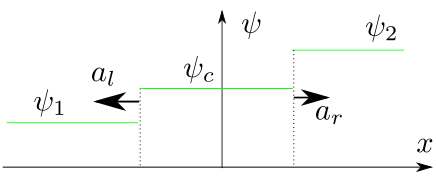
\includegraphics[width=80mm]{./help/Rieman2.png}
\caption{Задача Римана}
\label{rieman_problem}
\end{center}
\end{figure}

Тогда из законов сохранения поток на границе ячеек, в случае когда  $a_l$ и $a_r$ разных знаков

\begin{equation}
F^* = \frac{F_l a_r - F_r a_l + a_r a_l (U_r - U_l)}{a_r - a_l}
\end{equation}
 
Если $a_l$ и $a_r$ одного знака то мы просто сносим поток из ячейки справа или слева в зависимости от их знака.

\begin{equation}
\begin{aligned}
&W_{i+\frac12} = W_i,\text{  } a_l > 0\\
&W_{i+\frac12} = W_{i+1},\text{  } a_r < 0
\end{aligned}
\end{equation}

\begin{figure}[ht!]
\begin{center}
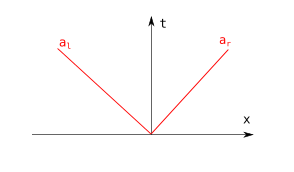
\includegraphics[width=80mm]{./help/Rieman1.png}
\caption{$a_r$ и $a_l$ разных знаков}
\label{rieman_problem2}
\end{center}
\end{figure}

Если же имеют $a_l$ и $a_r$ разные знаки то берем поток HLL

\begin{equation}
W_{i+\frac12} = \frac{W_i a_r - W_{i+1} r_l + a_r a_l (\psi_i - \psi_{i+1})}{a_r - a_l}
\end{equation}

За скорости распространения разрывов берем максимально и минимально возможную скорость звука. Запишем систему ввиде 

\begin{equation}
\frac{\partial \vec\psi}{\partial t}  + A \frac{\partial \vec\psi}{\partial x} = 0
\end{equation}

где

\begin{equation}
A = \begin{pmatrix}
 \frac{\partial W_l}{\partial \psi_l} &  \frac{\partial W_l}{\partial \psi_g} \\
 \frac{\partial W_g}{\partial \psi_l} &  \frac{\partial W_g}{\partial \psi_g} \\
\end{pmatrix}	
\end{equation}

Чтобы найти собственные значения решаем квадратное уравнение. Получаем два собственных значения

\begin{equation}
\begin{aligned}
\lambda_1 = \frac{- b - \sqrt{D}}{2}\\
\lambda_2 = \frac{- b + \sqrt{D}}{2}
\end{aligned}
\end{equation}

Ищем максимум и минимум собственных значений для всех возможных значений объемных долей: $a_l = min(\lambda_1(\theta_l, \theta_g)), \text{ } a_r = max(\lambda_2(\theta_l, \theta_g))$

\subsection{Блок энергии}
В блоке энергии вычисляется температура в каждой ячейке на новом временном слое. Выпишем уравнение энергии в Лагранжевых координатах

\begin{equation*}
\pd{} t \left((\psi_l c_l + c_s + \psi_g c_g)T\right) + \pd{} x \left(c_l T W_l + c_g T W_g - \lambda \theta_s \pd T x\right) = 0
\end{equation*}

Запишем для него схему Годунова???(Консервативную схему первого порядка).
\begin{equation}
T_i^{n+1} S^{n+1}_i = T_i^n S^{n}_i  - \tau\frac{Q^l_{i+\frac12} - Q^l_{i-\frac12}}{h} -\tau\frac{Q^g_{i+\frac12} - Q^g_{i-\frac12}}{h}  + \tau\frac{Q^{\lambda}_{i+\frac12} - Q^{\lambda}_{i-\frac12}}{h}
\end{equation}

где за $S^n_i$ обозначено $\psi_{l\text{ } i}^n c_l + c_s + \psi_{g\text{ } i}^n c_g$, за $S^{n+1}_i$ обозначено $\psi_{l\text{ } i}^{n+1} c_l + c_s + \psi_{g\text{ } i}^{n+1} c_g$ за $Q^l$ и $Q^g$ конвективные потоки тепла флюида и газа, за $Q^{\lambda}$ поток тепла за счет теплопроводности. 

Уже известны отношения объемных долей на текущем и предыдущем временном шаге, скорости фильтрации на границах ячеек и температура в ячейках на предыдущем шаге. Чтобы найти поток тепла на границе ячеек сносим температуру против потока.

\begin{equation}
\begin{aligned}
&Q^l_{i+\frac12} = W_{l\text{ } i+\frac12} T_{i+1}^n,\text{  } W_{l\text{ } i+\frac12} <0\\
&Q^l_{i+\frac12} = W_{l\text{ } i+\frac12} T_{i}^n,\text{  } W_{l\text{ } i+\frac12} >0
\end{aligned}
\end{equation} 

\begin{equation}
\begin{aligned}
&Q^g_{i+\frac12} = W_{g\text{ } i+\frac12} T_{i+1}^n,\text{  } W_{g\text{ } i+\frac12} <0\\
&Q^g_{i+\frac12} = W_{g\text{ } i+\frac12} T_{i}^n,\text{  } W_{g\text{ } i+\frac12} >0
\end{aligned}
\end{equation} 

Для потока тепла за счет теплопроводности нужно вычислить объемную долю твердой фазы на границе ячеек $\theta_{s\text{ } i+\frac12}$. Так как твердая фаза тяжелее всего, то она может двигаться только вниз. Поэтому сносим её справа

\begin{equation}
Q^{\lambda}_{i+\frac12} =  \lambda \theta_{s\text{ } i +1} \frac{T_{i+1}^n - T_i^n}{h} 
\end{equation}

\section{Результаты расчетов}


\section{Расчеты на лабораторном симуляторе}


\section{Не вписано}
Можно переписать систему в виде
\begin{equation}
\frac{\partial \vec\psi}{\partial t}  = A \frac{\partial \vec\psi}{\partial x}
\end{equation}

где
\begin{equation}
A = \begin{pmatrix}
 \frac{\partial W_l}{\partial \psi_l} &  \frac{\partial W_l}{\partial \psi_g} \\
 \frac{\partial W_g}{\partial \psi_l} &  \frac{\partial W_g}{\partial \psi_g} \\
\end{pmatrix}	
\end{equation}

\begin{equation}
\begin{aligned}
&\pd{W_l}{\psi_l} = -\frac{\psi_l (2 \psi_g + 2 - \psi_l) (\psi_g (\rho_g-\rho_l)-\rho_l+\rho_s)}{\eta_l (\psi_g+\psi_l+1)^4} g\\
&\pd{W_l}{\psi_g} = -\frac{\psi_l^2 (\rho_g (\psi_l + 1 - 2 \psi_g)+\rho_l (2 \psi_g + 2 - \psi_l)- 3 \rho_s)}{\eta_l (\psi_g + \psi_l + 1)^4}g\\
&\pd{W_g}{\psi_l} = -\frac{\psi_g^2(\rho_g (2\psi_l + 2 - \psi_g)+\rho_l (\psi_g - 2 \psi_l + 1) - 3 \rho_s)}{\eta_g (\psi_g + \psi_l + 1)^4}g\\
&\pd{W_g}{\psi_g} = -\frac{\psi_g (2\psi_l + 2 - \psi_g) (\psi_l (\rho_l -\rho_g) - \rho_g + \rho_s)}{\eta_g (\psi_g + \psi_l + 1)^4}g\\
\end{aligned}
\end{equation}

Ищем собственные значения
\begin{equation}
\lambda^2 - (W_1 + W_4)\lambda + W_1 W_4 - W_3 W_2 = 0	
\end{equation}
\begin{equation}
D = (W_1 + W_4)^2 - 4(W_1 W_4 - W_3 W_2)	
\end{equation}


\end{document}